\vspace{-0.2cm}

The problem of taxonomy classification of product titles is central to an e-commerce organization. 
Large online e-commerce companies usually obtain millions of new listing feeds per month from several hundred merchants subscribed to use proprietary ``publish $\rightarrow$ search $\rightarrow$ buy'' platforms specific to each of these companies. 
The ease of use, control on data quality and organization and functionality of these platforms are the key factors for differentiating the success of the revenue generation model for the companies.

The sale of product listings within an e-commerce platform is critically dependent upon end users being able to search for the correct product using some minimal to advanced search functionality provided by the developers of the platform. 
In this paper we differentiate products from product listings using a simple example. 
Consider a product with a title of ``\textit{Wilson tennis racket Level 3 signed by Federer}''. 
Merchant \textbf{A} can list this product with a title of ``\textit{Wilson tennis racquet Level 3 Roger Federer}''' and with a list price of \$80 while merchant \textbf{B} can list the same product with its original title but with a list price of \$72.
The e-commerce platform keeps track of these two product items as two different listings although they are the same product after some title text disambiguation.
Similar examples occur in thousands for product titles having the same title text but differing in price and/or other fields.
Title text disambiguation in absence of any global identifier for products is also a core-problem in e-commerce platforms that follow an online marketplace model, but we do not address that problem here.
In this paper, we will refer to product listings as listings henceforth. 

Most e-commerce companies keep track of high Gross Merchandise Sales (GMS) products and tune search results to queries conditional on GMS and other meta features such as clickstream as well as  content specific features.
One such critical meta feature is the taxonomy classification of listings.
On a web search platform, categories of search results have already been used to improve web query classification \cite{Ganti10} and such kind of query classifications are also very useful for product search engines.
Further, clues from taxonomies have are very useful in user persona detection and targeted campaigns, recommendations, clustering of  ranked lists of listings and many other applications.

\begin{figure}[ht]
	\centering
	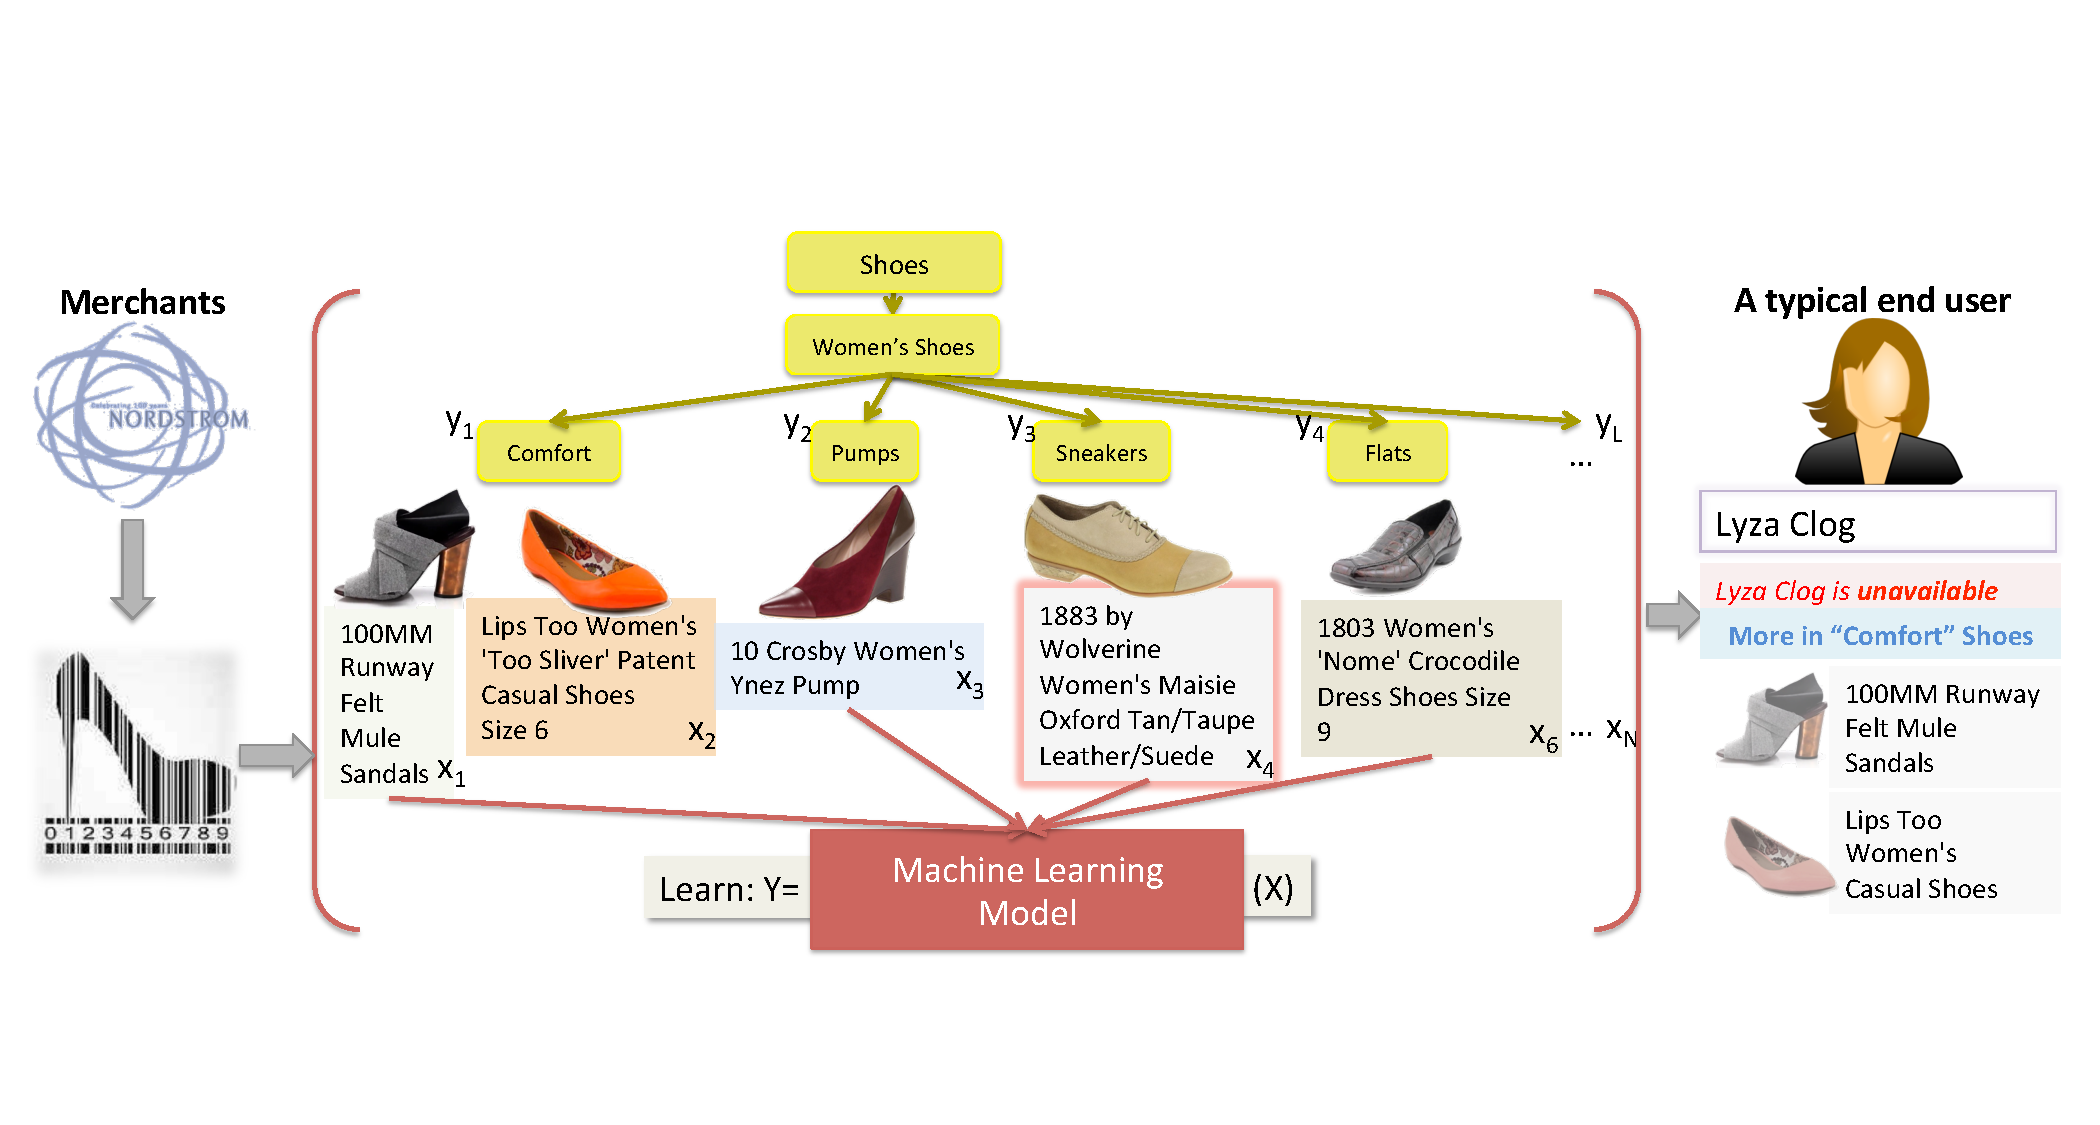
\includegraphics[width=0.9\textwidth]{images/push-pull}
	\vspace{-0.2cm}
	\caption{{\small Merchants push new listings to a data organization and search platform. The listings are then annotated in various ways including a core taxonomy categorization component. The indexed listings together with the annotations influence search and other data organization algorithms. The relevance of the information that end users pull from the indexing platform determines the eventual conversion and revenue generation effectiveness of the e-commerce platform. In this example, it can be easily observed how taxonomy classification can be very helpful in identifying the intent of the query.}}
	\label{Fig:push-pull}
	\vspace{-0.6cm}
\end{figure}

In this paper, we focus on taxonomy classification of listings in order to solve problems arising in the scenario described in Fig. \ref{Fig:push-pull}.
Generally, merchants interested in publishing their listings to an online e-commerce platform, pushes their feed to an intelligent indexing engine which then are ready to be consumed by the end user in a variety of ways.
Scalable and accurate taxonomy categorization of listings is often among the earliest core annotation steps for these platforms.
Feeds usually come in at 10-20 million listings/day for mid scale e-commerce companies.

Our problem here is to classify each test instance (listing), $\bm{x}_m$ in Fig. \ref{Fig:push-pull}, into the correct taxonomy branch, $\bm{y}_l$ e.g. ``\textit{Shoes $\rightarrow$ Women's Shoes $\rightarrow$ Comfort}''.
In order to reduce classification calls at runtime and to prevent error snowballing effect of a cascading hierarchical classifier, we solve the taxonomy classification problem in two levels.
For example, a test listing is first classified into one of the level one classes shown in the Fig. \ref{Fig:push-pull} e.g. ``\textit{Shoes}''.
It is then classified by the classification model corresponding to the level one taxonomy subtree identified by the predicted level one root node (e.g. ``\textit{Shoes}'').
A similar approach is taken in \cite{Shen12} but their second level nodes have 4.6 to 3.3 branches on average.
We instead use the hierarchical structure given to us by taxonomists.
As noted in \cite{Julian15}, not all listings reside in leaf nodes, however, for our case, we consider $\bm{y}_l$ to be the label of the node where $\bm{x}_n$ resides, up until the root node of the taxonomy tree i.e the corresponding branch.

In large e-commerce companies that follow the marketplace models of business to business to customer (B2B2C) commerce, such as Rakuten, maintaining an unified product taxonomy a.k.a product catalog is very difficult. 
This can happen for many reasons including updates to taxonomies due the changing product lines, cross-border trading and more importantly acquisitions of external companies that are niche.
Each of the acquired companies has their own taxonomies and although they are merged under a common parent company, they operate as independent Business Units (BUs)  for some time with their own data feeds and data organization algorithms.
In this paper, we perform experiments on listings data from two such BUs -- BU1 and BU2 -- belonging to Rakuten USA Inc.
that is managed by Rakuten Ichiba, the largest e-commerce company in Japan.

The main contributions of our work are three folds -- 
1) We conduct large scale experiments on taxonomy classification of product titles using state-of-the-art classifiers and conclude that the performances of GBTs and CNNs are much superior and comparable using only word unigram features (Section \ref{Sect:results}) which also makes feature extraction very fast at runtime. 
2) We make use of correspondence LDA models to identify patterns of data corruption (Section \ref{Subsect:BU2-noise-analysis}) in the training set that has been obtained from product page crawls in the wild. 
3) Additionally, we show that including the list price and the root node of navigational breadcrumbs whenever available, boost prediction performance significantly (Section \ref{Subsect:BU2-classification-improve-list-price}).


